\documentclass{article}
\usepackage{amsmath}
\usepackage{graphicx}
\usepackage{hyperref}

\title{Hawk-Dove Game Simulation with Resource Dynamics}
\author{Geoffrey Wang}
\date{\today}

\begin{document}

\maketitle

\begin{abstract}
This report details the implementation and analysis of a Hawk-Dove game simulation with resource dynamics. The simulation models the strategic interactions between individuals with different strategies (Hawk, Dove, and Mixed) under resource constraints. The dynamics of resource availability and strategy selection are explored through various parameters, including the cost of conflict, the value of resources, and the rate of resource regeneration.
\end{abstract}

\section{Introduction}
The Hawk-Dove game is a classic model in evolutionary game theory that describes the conflict between two strategies: Hawk (aggressive) and Dove (peaceful). This model is used to study how these strategies compete under different conditions, particularly in the context of limited resources. In this project, we extend the traditional Hawk-Dove game by introducing resource dynamics, where the availability of resources influences the outcomes of strategic interactions.

\section{Methodology}
\subsection{Model Overview}
The model consists of a population of individuals who adopt one of three strategies:
\begin{itemize}
    \item \textbf{Hawk}: An aggressive strategy that always fights for resources.
    \item \textbf{Dove}: A peaceful strategy that avoids conflict and shares resources.
    \item \textbf{Mixed}: A strategy that randomly switches between Hawk and Dove.
\end{itemize}

The interactions between individuals are governed by the following parameters:
\begin{itemize}
    \item \textbf{Resource Value (V)}: The value of the resources being contested.
    \item \textbf{Fight Cost (C)}: The cost incurred by individuals when engaging in a conflict.
    \item \textbf{Initial Population Fractions}: The initial proportion of the population adopting each strategy (Hawk, Dove, Mixed).
    \item \textbf{Mutation Rate}: The probability that an individual will randomly change its strategy in each generation.
    \item \textbf{Initial Resource Amount}: The total resources available at the start of the simulation.
    \item \textbf{Renewable Resource Percentage}: The fraction of resources that are renewable, as opposed to non-renewable.
    \item \textbf{Renewable Recovery Amount}: The amount of renewable resources that are replenished each generation.
\end{itemize}

\subsection{Simulation Process}
The simulation proceeds in discrete generations. In each generation, individuals are paired to interact according to their strategies. The outcomes of these interactions depend on the resources available and the strategies adopted:
\begin{itemize}
    \item \textbf{Hawk vs. Hawk}: Both individuals incur a cost (C) and share the remaining resources.
    \item \textbf{Hawk vs. Dove}: The Hawk individual takes all the resources, while the Dove gets none.
    \item \textbf{Dove vs. Dove}: Both individuals share the resources equally.
    \item \textbf{Mixed}: A Mixed strategy individual chooses either Hawk or Dove with equal probability.
\end{itemize}

After each generation, the resources are updated:
\begin{itemize}
    \item Non-renewable resources decrease based on the total resources consumed.
    \item Renewable resources are replenished up to a maximum value.
\end{itemize}

\subsection{Mutation Mechanism}
To introduce variability and prevent stagnation in strategies, a mutation mechanism is included. In each generation, there is a small chance (defined by the mutation rate) that an individual will change its strategy to either Hawk, Dove, or Mixed.

\section{Experimental Results}
The simulation was run with the following parameters:
\begin{itemize}
    \item Resource Value (V): 50
    \item Fight Cost (C): 100
    \item Population Size: 100
    \item Initial Hawk Fraction: 0.3
    \item Initial Dove Fraction: 0.3
    \item Initial Mixed Fraction: 0.4
    \item Number of Generations: 1000
    \item Mutation Rate: 0.005
    \item Initial Resource: 1000
    \item Renewable Resource Percentage: 0.7
    \item Renewable Recovery Amount: 10
\end{itemize}

The results are shown in the figures below, where the top plot shows the fractions of individuals adopting each strategy over generations, and the bottom plot shows the available resources over time.

\begin{figure}[h]
    \centering
    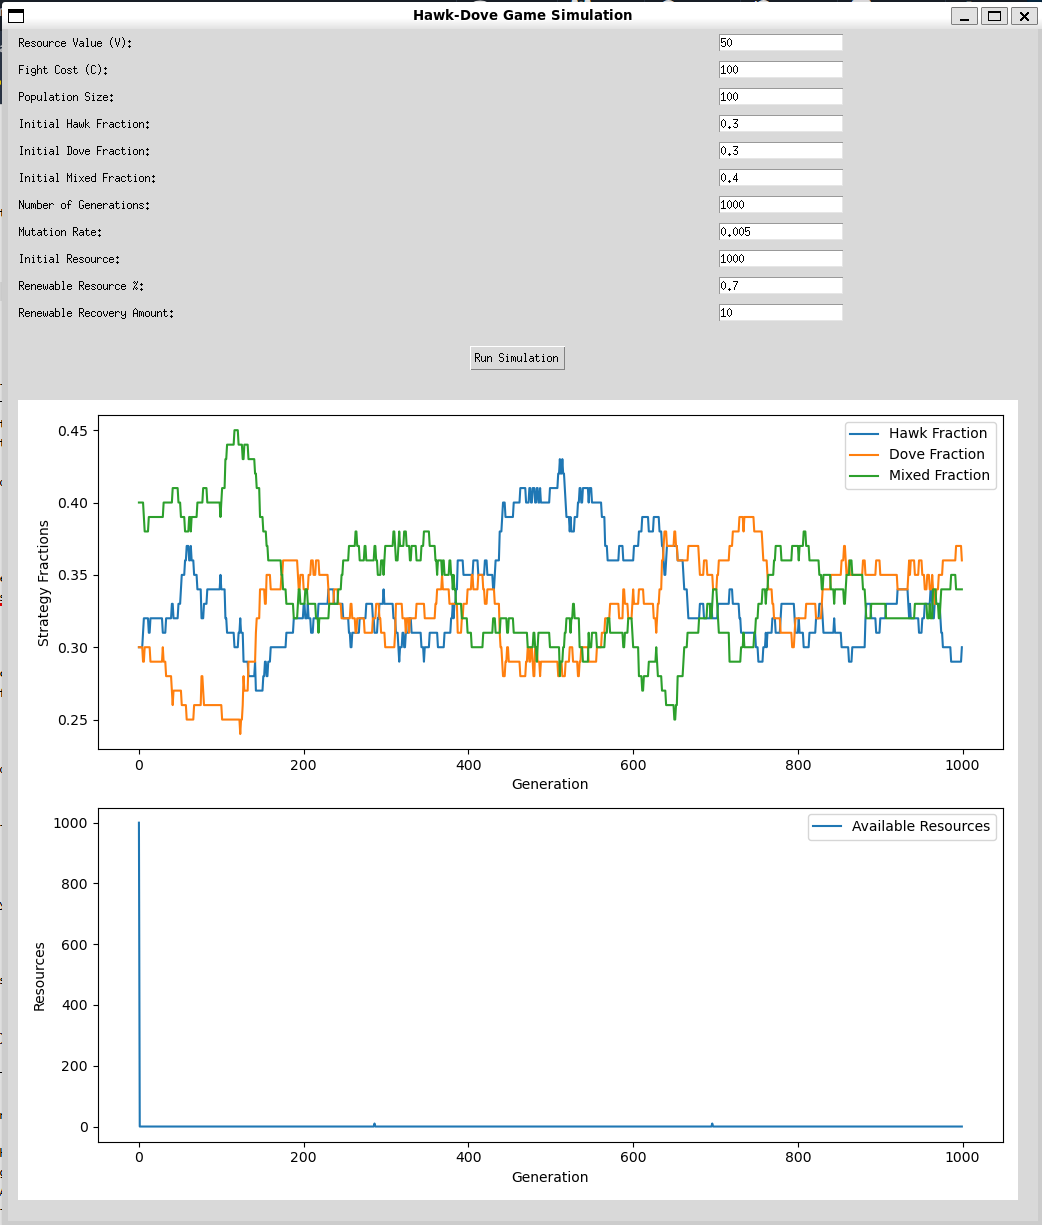
\includegraphics[width=0.8\textwidth]{HawkDoveGame.png}
    \caption{Strategy fractions and available resources over generations.}
    \label{fig:results}
\end{figure}

\section{Discussion}
The simulation results highlight several key dynamics:
\begin{itemize}
    \item \textbf{Strategy Dynamics}: The fractions of Hawk, Dove, and Mixed strategies fluctuate over time, influenced by resource availability and the costs of conflict.
    \item \textbf{Resource Depletion and Recovery}: The resource dynamics play a critical role in shaping the strategies. As resources deplete, aggressive strategies like Hawk become less viable, leading to a potential rise in Dove and Mixed strategies.
    \item \textbf{Mutation Effects}: The introduction of mutation prevents the population from becoming stagnant and allows for the exploration of different strategy combinations.
\end{itemize}

In some scenarios, the resources were quickly depleted, leading to a stable state where no significant strategy changes occurred. In others, the resource replenishment allowed for continuous competition and strategy shifts.

\section{Conclusion}
This project demonstrates how the Hawk-Dove game can be extended to include resource dynamics, providing a richer model for studying strategic interactions in environments with limited resources. The simulation shows that resource availability and regeneration significantly impact the strategies adopted by individuals. Future work could explore different mutation rates, resource regeneration rates, and the introduction of additional strategies.

\section{References}
\begin{itemize}
    \item Maynard Smith, J., \& Price, G. R. (1973). The logic of animal conflict. Nature, 246(5427), 15-18.
    \item Axelrod, R., \& Hamilton, W. D. (1981). The evolution of cooperation. Science, 211(4489), 1390-1396.
\end{itemize}

\end{document}
